\documentclass[a4paper]{article}

\usepackage{parskip}
\usepackage{setspace}
\usepackage{fullpage}
\usepackage{graphicx}
\usepackage{float}
\usepackage[justification=centering]{caption}


\begin{document}

\title{Product Management, Feedback and Evaluation}
\author{Andrew Higginson \and Bryan Liu \and Jia Guang Choo \and Emma Hulme \and 
Timothy van Bremen \and Thomas Taylor-Hall}
\date{\today}
\maketitle

\setcounter{table}{0}
\linespread{1.15}

\section{Project Introduction}
As part of the renovation of the William Penney Building on the Sherfield 
walkway, interactive screens are to be installed. Mounted inside the building,
four projectors will simultaneously display content onto floor to ceiling glass
panels that are visible to passers-by. Also, an 84-inch 4K resolution touch 
screen is to be mounted by the entrance doors. 

Our project consists of developing an ``App Store" for uploading interactive 
content and visualisations to be displayed on the four projected screens. 
Administrators will also be able to use this system to moderate and schedule 
content. Finally, we will be developing a playout system to show the content 
on multiple screens in multiple resolutions.

\section{Relationships and Feedback}
Early on we identified that the main stakeholder in our project is our supervisor David. The core of our project is the scheduling component, which he would operate as an administrator, and so his opinion of the overall design of the project was critical. We also identified our second class of stakeholder, those who browse the visualisation catalogue and submit visualisations and adverts. Their stake is relatively large as without their full engagement and satisfaction, the variety of content being shown will remain small. Finally those see the visualisations being played out. Whilst this final set of users are important, their stake is relatively small, in that all they need to see is the content being played out successfully.

Our relationship with our supervisor David has consisted of weekly 
meetings, and emails if appropriate. Finally, we explain what features are in progress/to be done over the next week so David is 
always kept in the loop. We tended to keep discussions fairly high-level, and only discussed implementation details/technologies when asked to do so, or when we felt that it was important to the discussion. We did this to mimic the scenario of David being our client, but also so that discussions we not biased towards any kind of implementation, so that we fitted our implementation around the best ideas, and not the other way around.

\begin{figure}[H]
  \begin{minipage}{0.49\textwidth}
    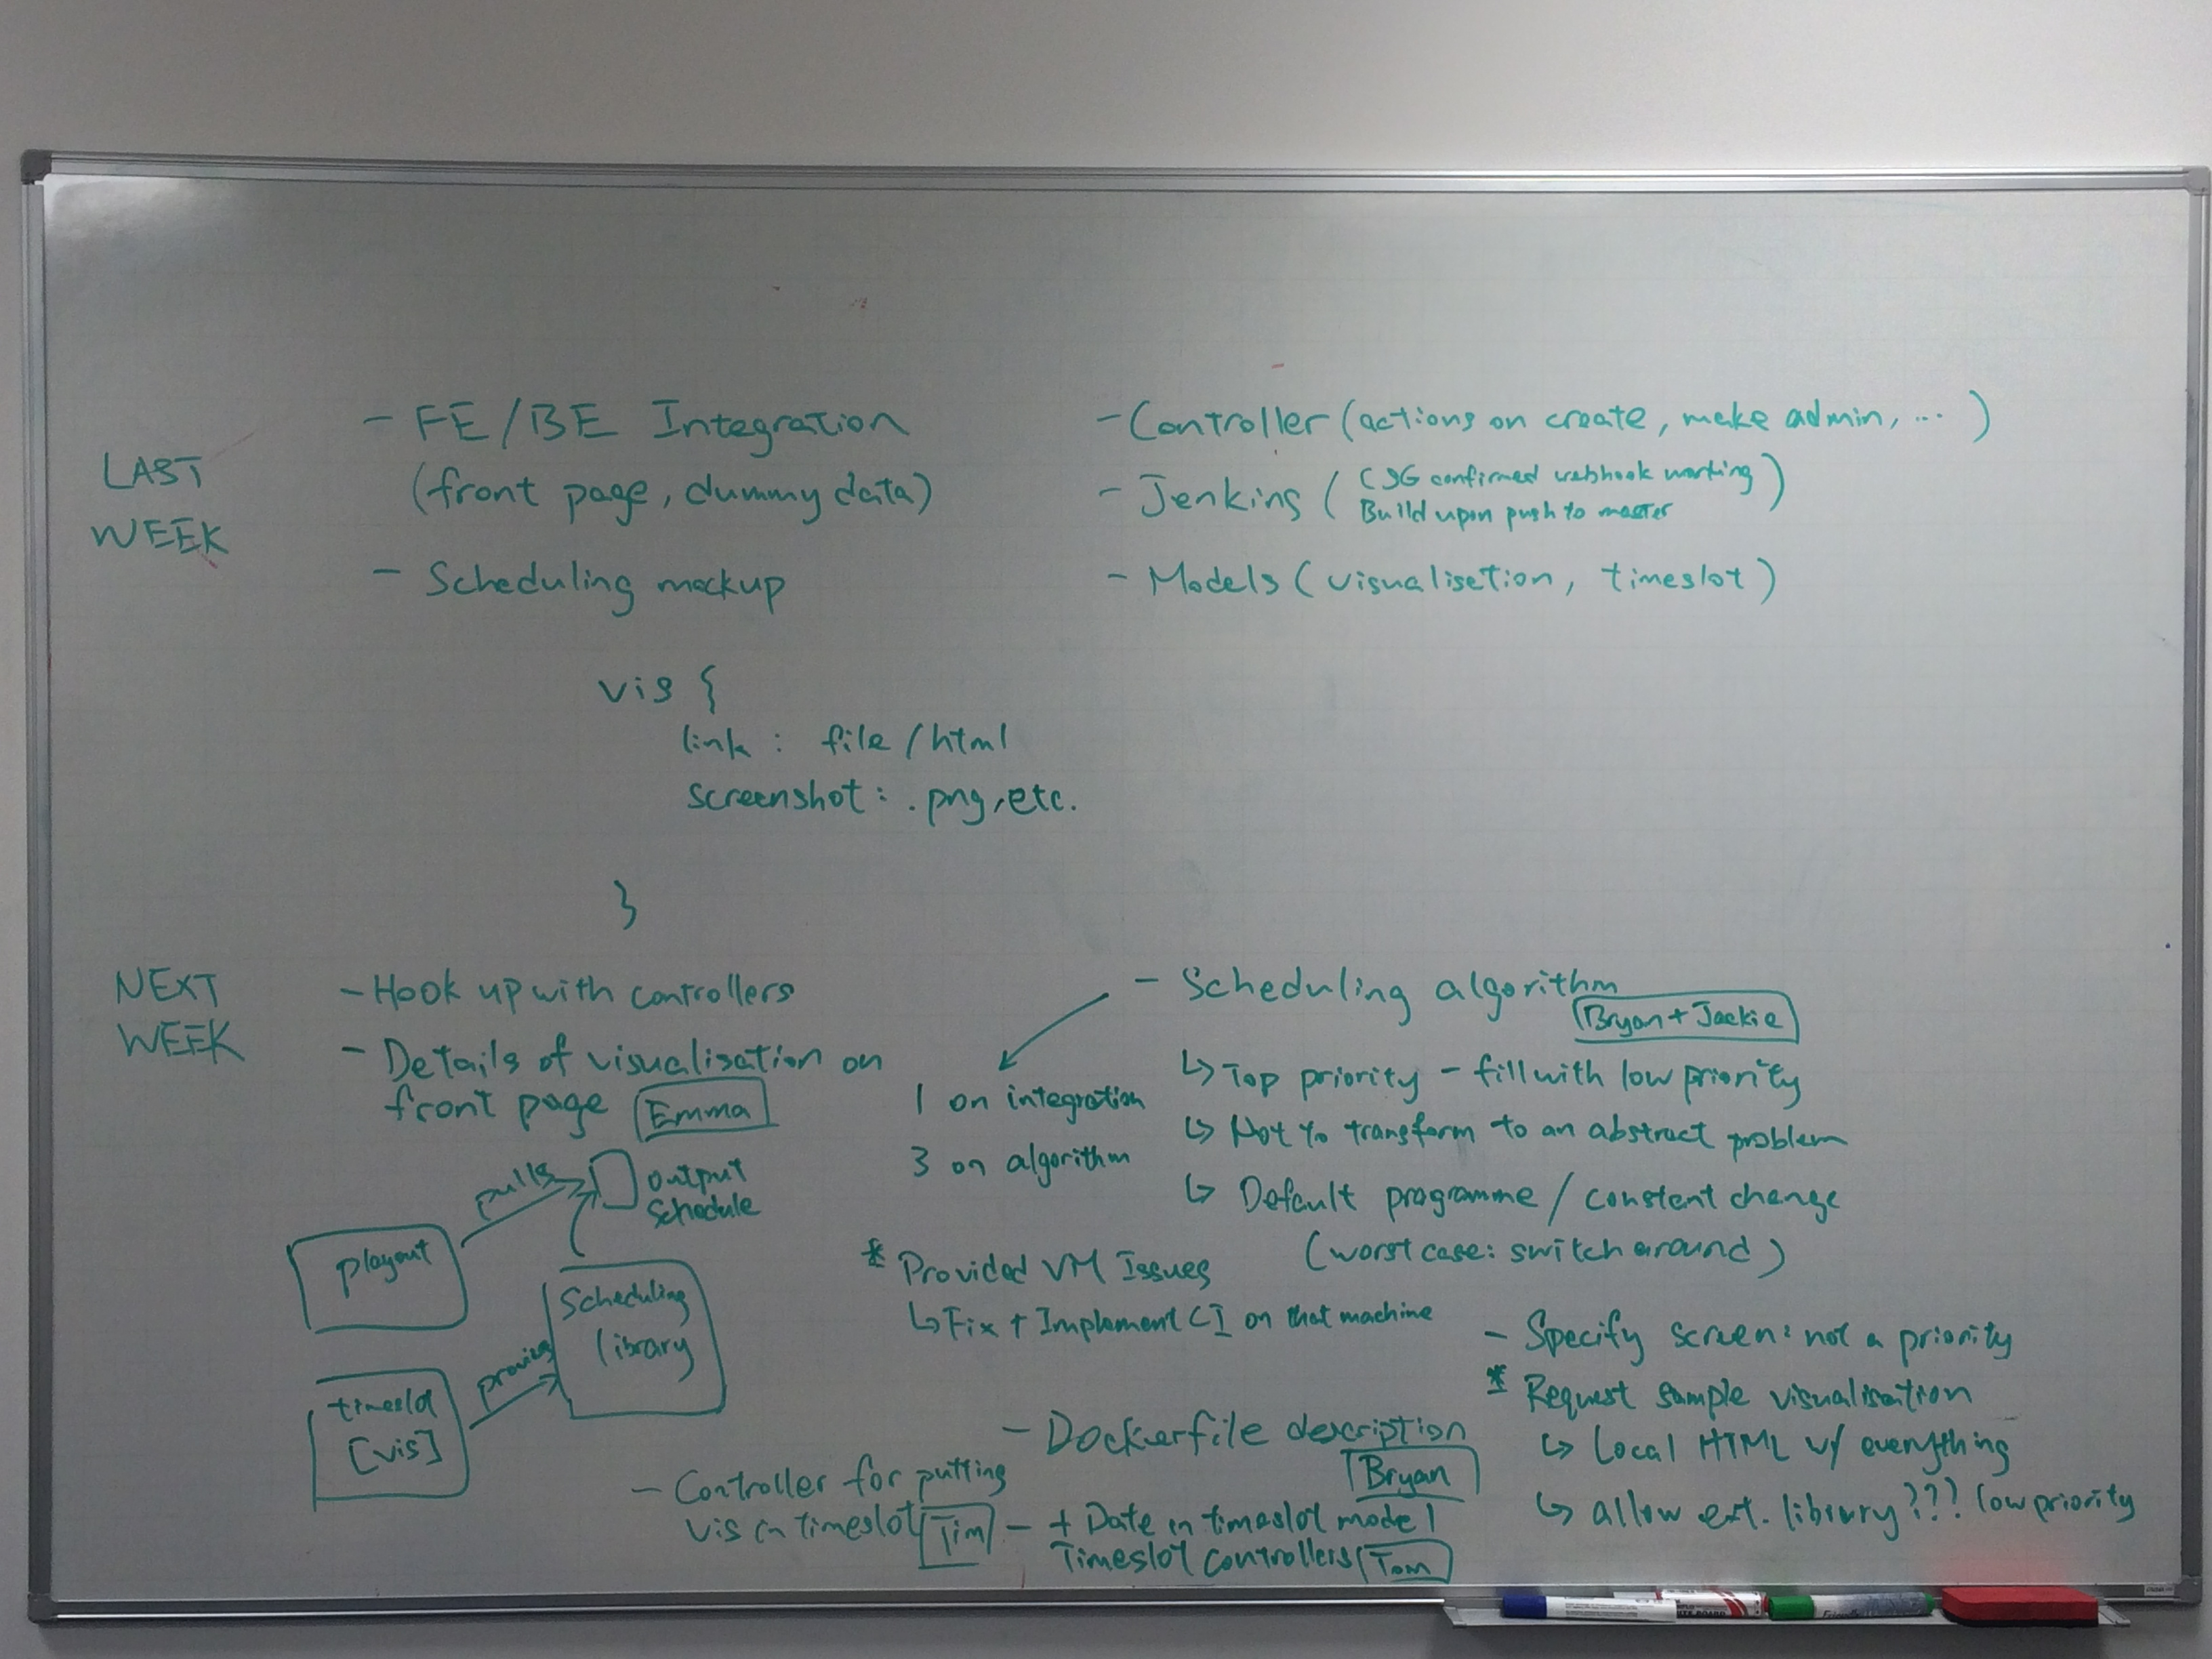
\includegraphics[width = \textwidth, trim = 0 0.4cm 0 1.6cm, clip]{./evaluation/meeting-board2.jpg}
  \end{minipage}
  \begin{minipage}{0.49\textwidth}
    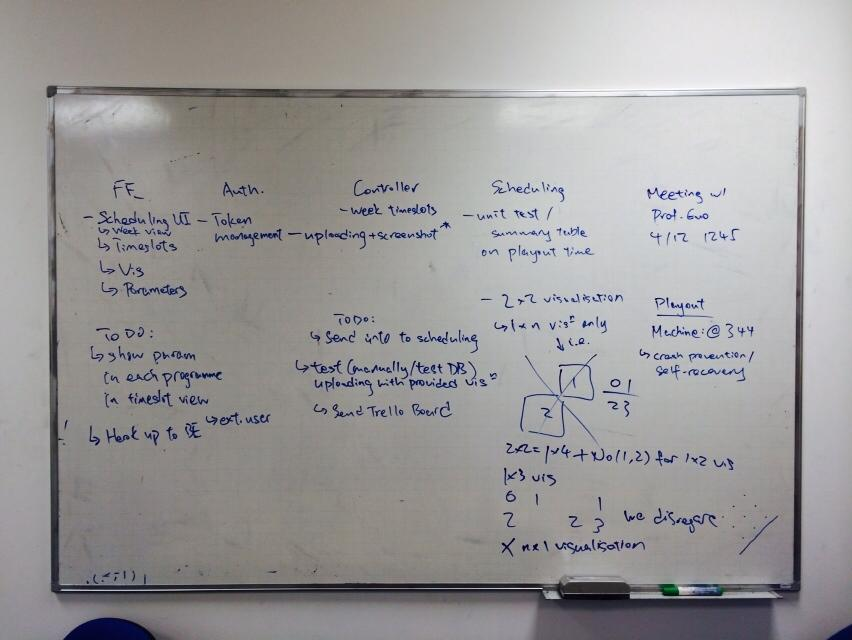
\includegraphics[width = \textwidth, trim = 1.2cm 1.5cm 1.2cm 2.5cm, clip]{./evaluation/meeting-board.jpg}
  \end{minipage}
  \caption{Meeting notes showing feedback from David (our supervisor) and group progress \\
                    after sprint cycles 2 (left) and 4 (right).}
  \label{fig:meetingboard}
\end{figure}

We have also received some representative model data to seed our database, 
instead of using dummy data. This was provided by David and will also be 
used to test submission, moderation and display features of our system.

For example, after we showed David mockups of the scheduling screen, he said that 
he wanted priorities associated with each visualisation to be shown. We agreed as a 
group that this would be easy to implement, and assigned the task to an appropriate
group member on Trello. 


\section{Product Requirement, Value \& Impact}
In the first week of beginning our project, we met with our supervisor 
David to draw out the initial components. Initially, these were general
requirements that we divided into user, admin and interface 
requirements. We later sent these requirements to David so he could check
they were satisfactory and have them for his records. He was happy with 
these and did not modify them.



\begin{figure}[H]
  \centering
    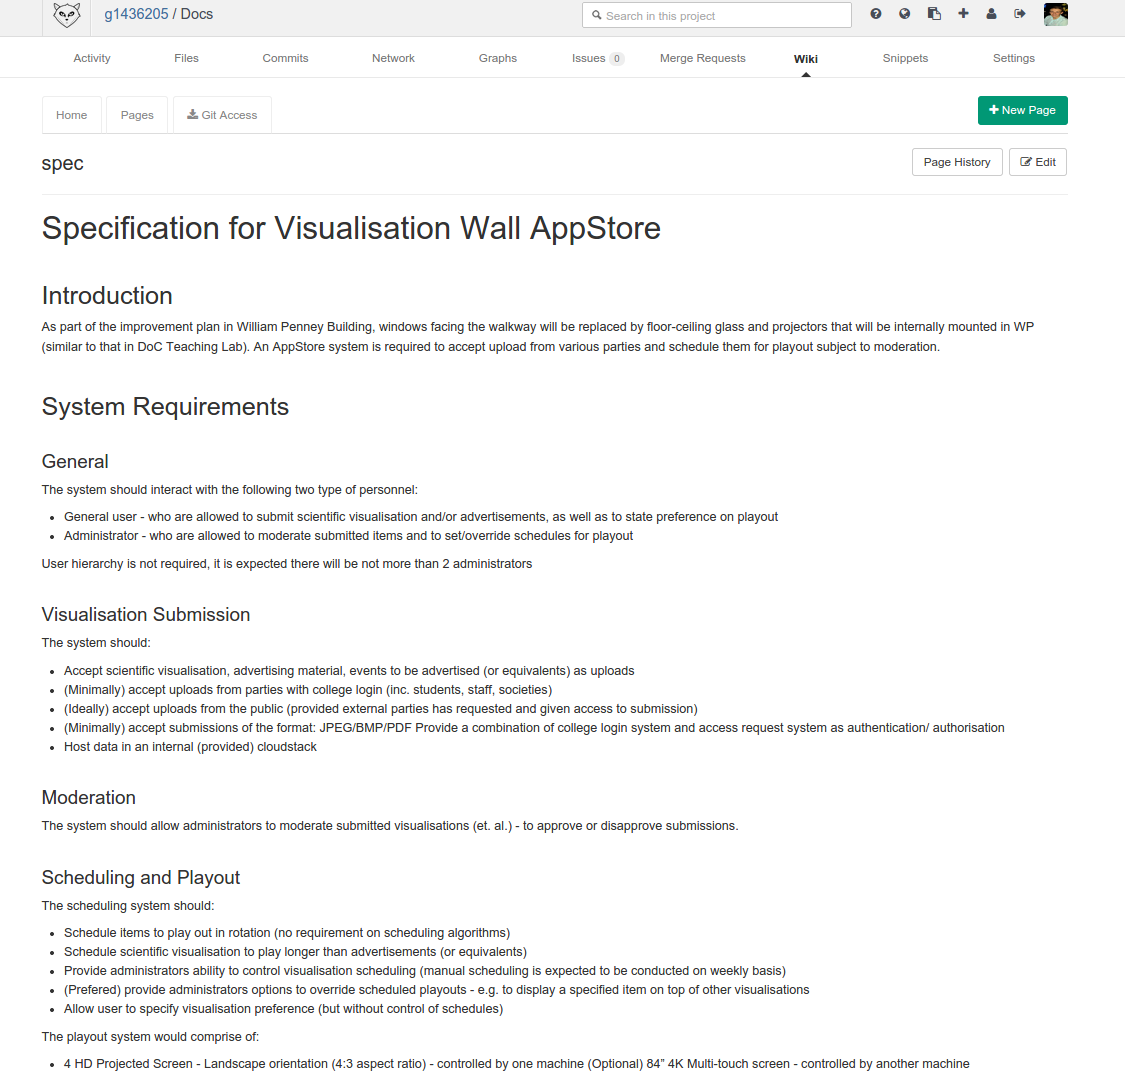
\includegraphics[width = 0.5\textwidth]{./evaluation/specs.png}

  \caption{Initial specifications on shared repository.}
  \label{fig:specs}
\end{figure}

\subsection{Value Proposition}
\begin{figure}[H]
   \begin{center}
      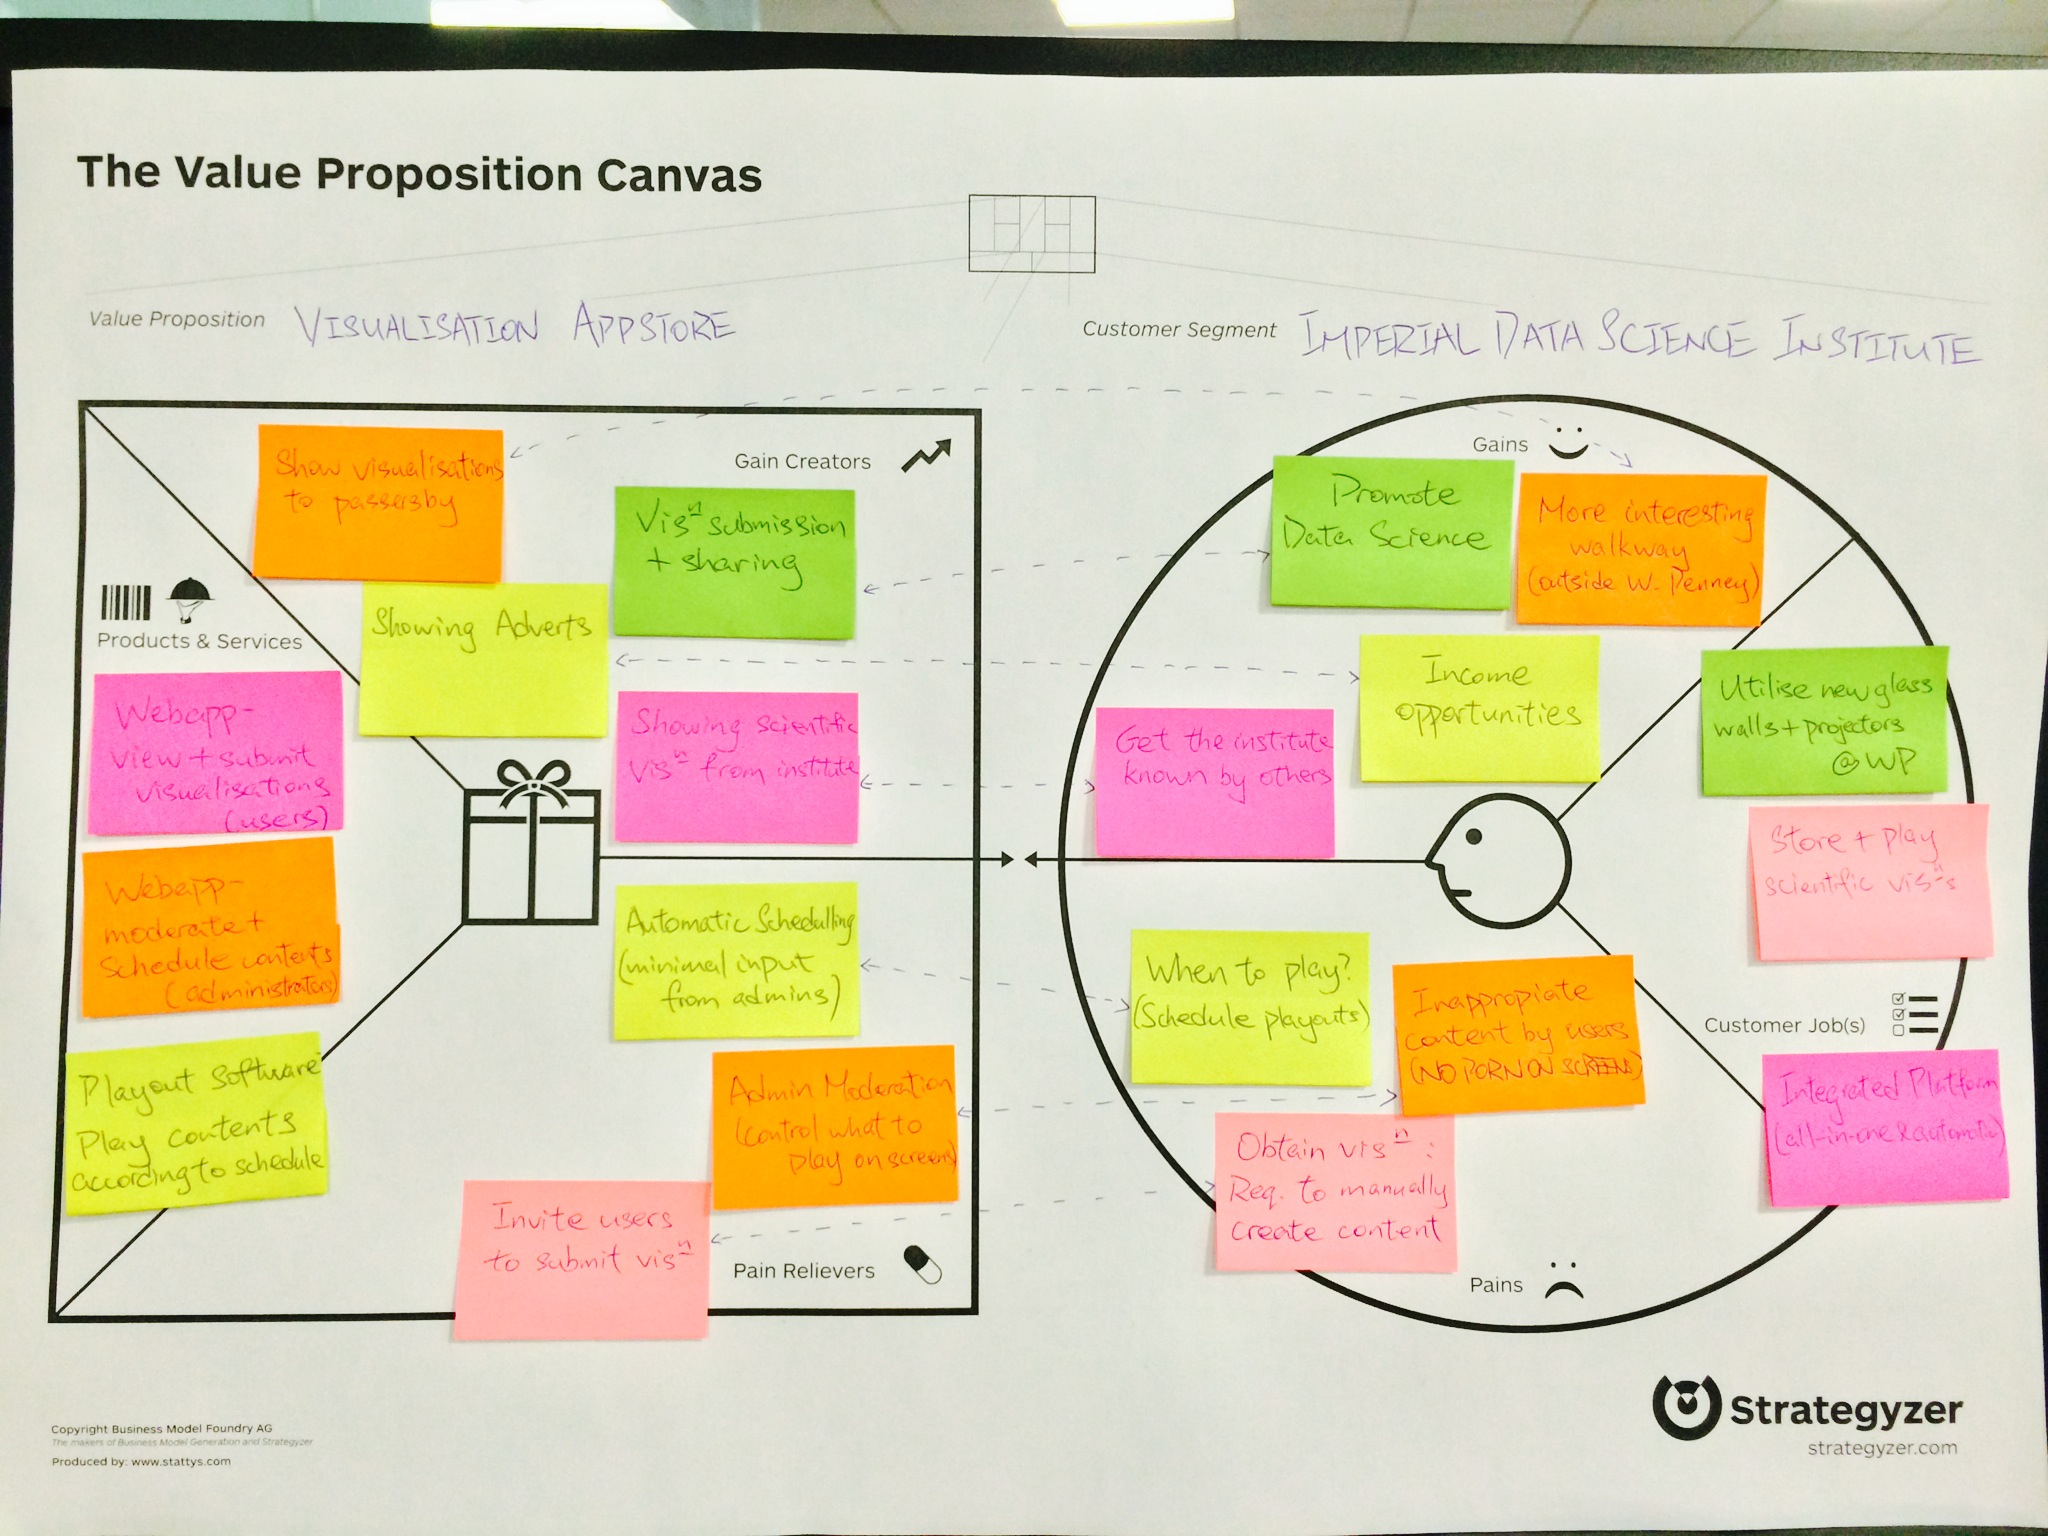
\includegraphics[width = 0.99\textwidth, trim = 1cm 6.5cm 1cm 4.5cm, clip]{./evaluation/value_prop_canvas.jpg}
   \end{center}
   \caption{Value proposition canvas for our client (Imperial Data
            Science Institute).}
   \label{fig:valpropcanvas}
\end{figure}



\section{Task Management}
In the coming weeks, we then clarified and expanded these requirements as 
a group. This allowed us to discuss implementation and technical details
of specific features.


During development, we are constantly looking at the requirements for all of our stakeholders, which 
we have stored in a shared document. In our weekly scrums, we have 
presented the work we have done and discuss whether the project is on the 
right track. In our discussions, David has refined how he wants our
scheduling algorithm to schedule visualisations for a particular time. 



We have been prioritising tasks using our Trello board with different
columns. In addition to this, we have been constantly communication both 
in person and online, to make sure members are implementing assigned tasks
in appropriate times. We have been actively encouraging use of the Trello 
board to update the group when tasks have been completed. This way, 
we don't have to constantly ask or look at code to see if a feature has 
been implemented. If appropriate, group members working on the backend
have been using an internal wiki on gitlab to provide information about
routing, controller actions and parameters. 


\begin{figure}[H]
  \centering
    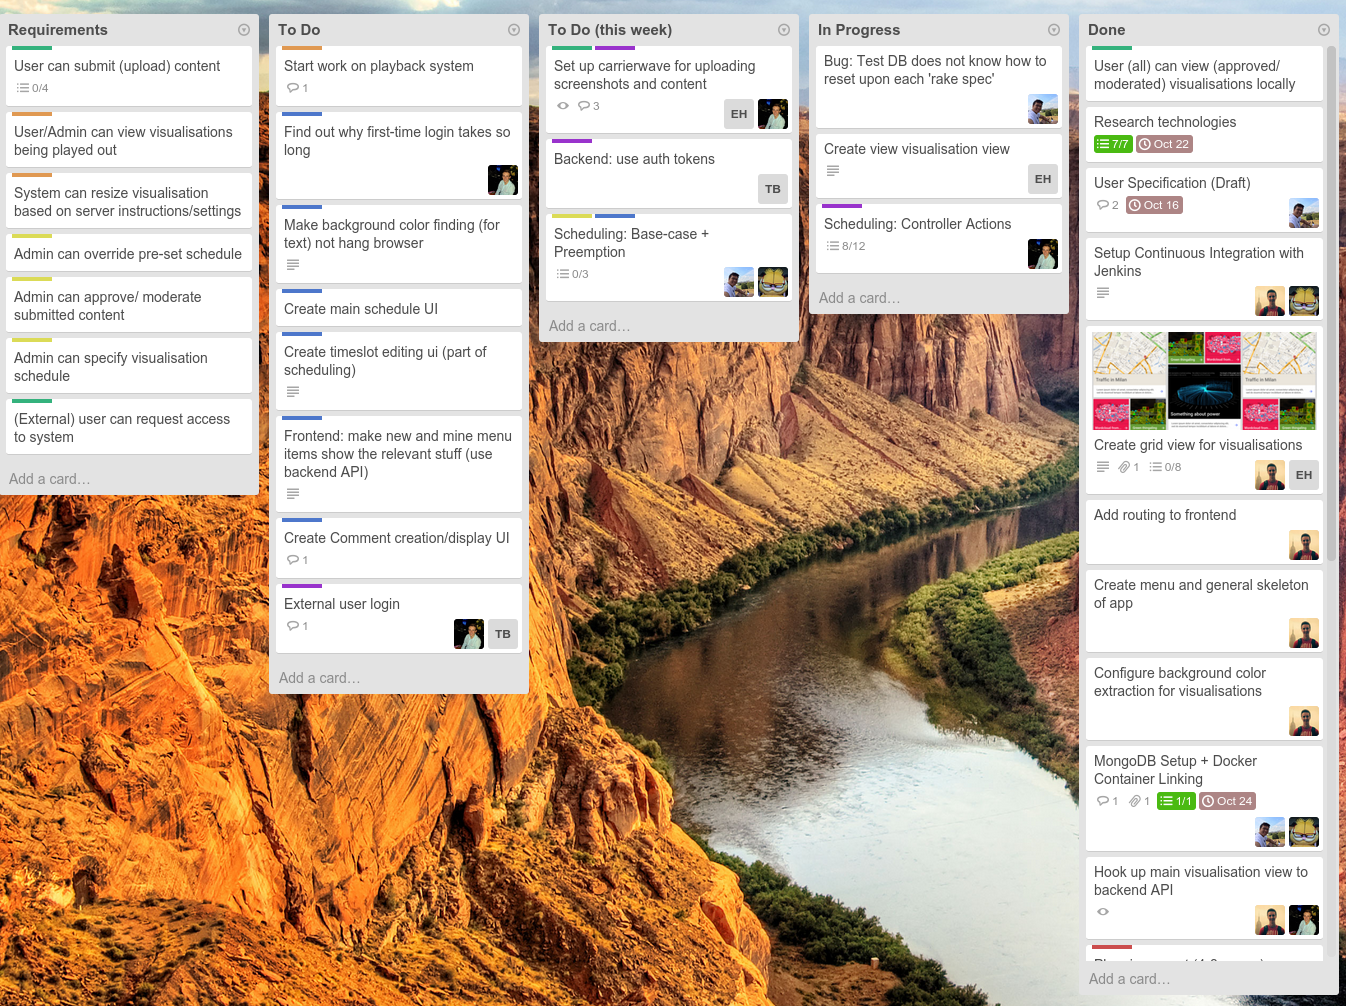
\includegraphics[width = 0.5\textwidth]{./evaluation/trello-columns.png}

  \caption{Priority columns on our Trello board.}
  \label{fig:columns}
\end{figure}


\begin{figure}[H]
  \centering
    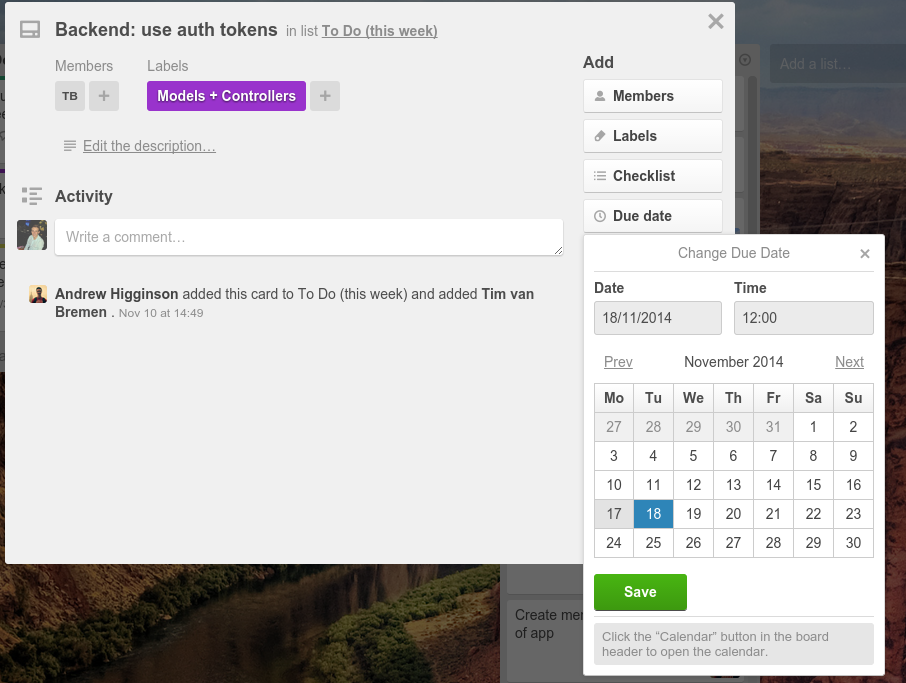
\includegraphics[width = 0.5\textwidth]{./evaluation/trello-due-date.png}

  \caption{Setting a due date for a particular task.}
  \label{fig:deadline}
\end{figure}




\subsection{Story Splitting}
While some of the requirements require only a few hours effort. We believe
it would be highly unlikely to implement some of the features within an
iteration. In such cases we have splitted the features into multiple units and
implement them in different iterations based on their priority.

An example would be on the user story
 "As a user, I want to access the platform via a set of
credentials so that I can upload visualisation (user)/ perform moderation and
scheduling (administrator)". We consider this to be technically challenging
if we consider all possible users and decided to split it into:

\begin{itemize}
  \item As an internal user (student/staff at Imperial), I want to access the 
        platform via college login so that I can upload/ moderate and schedule
        without memorising an extra set of credentials.
  \item As an external user, I want to access the platform via some kind
        of access request system so that I could participate in visualisation
        sharing as well. 
\end{itemize}

While being reduced in size, splitting the story has also helped us to 
further understand the needs
of different groups of users. We have decided to implement the former requirement
first as other features, such as scheduling and moderation, would require
a working version of access control, thus having a higher priority.
The later requirement can then be scheduled
to be carried out in parallel with the mentioned features.

\subsection{Spikes - Experiments with new technologies}
Throughout development, we have also devote a small proportion of time to
experiment on technologies involved in later iterations. This allows us to
better understand the complexity we will face and react accordingly.

While we have scheduled to implement the playout system in iterations 5 and 6
(the last two iterations),
investigation on relevant technologies, including QT and its adapters, were
made from iteration 2. By performing preliminary research, it allows 
us to confirm that 2 weeks would be a reasonable estimate in system 
implementation. Furthermore, we believe the investigation would result 
in a more gentle learning curve, and reduces the risk for development 
grinding to a halt as team members would
at least have some basic knowledge on QT and some code segments are produced.

Not all spikes brings good news - investigation on Kerberos login libraries has
revealed that the adapter for Flask (with Python) is actually broken.
Though being required to scrap the entire implementation, the spike allows us
to switch development language early and thus avoids incurring high 
cost further into development.

\section{Building the right thing - Assumption Validation}
Given the tight time constraints for the entire project, we agreed to collect
user feedback as soon as the project commences. This ensures the team
is building the right thing which our client needs.


\subsection{User interface mockups}
A release cycle in our project generally takes the following form. Before implementing a particular part of our project, we begin with creating mockups (figure \ref{fig:mockup}). These are relatively quick to produce and allow us to quickly think through the design of our project, with being tied down to any implementation details which would affect our thinking. After completion, we then show the mockups to the main stakeholder in the project, our supervisor David, who gives us feedback/changes. Once a general design is settled on, within that week's sprint cycle, we complete the main implementation of the UI, but only do so up to the point of it being useful to show how it would be used. It is not yet interfacing with the backend, and hence small changes at this point are simple to do, with the following week's sprint cycle involving 'hooking' up this UI prototype and our backend.\\

We also make sure that this prototype is in some way, seeded with some dummy/representative data, so that it is clear how each part of the project will operate in practice.\\

This way of working allows us to 'pivot' many times, and with minimal overhead of reimplementation, as it allows us to identify problems, or learn more about the issue we are trying to solve, before we write large volumes of code which may end up to be not useful. The fact that we have this lean approach also \textbf{encourages us} to pivot more often, as there is no reason not to do so.

During a meeting with David, our supervisor, he mentioned after going 
through the mockups that it would be a good if we could show the priorities
associated with each visualisation in timeslot view, even if the visualisation
is not selected.
%TODO: consider moving the  
We agreed as a group that this would be easy to implement, and assigned the 
task to an appropriate group member on Trello.

\begin{figure}[H]
   \begin{center}
      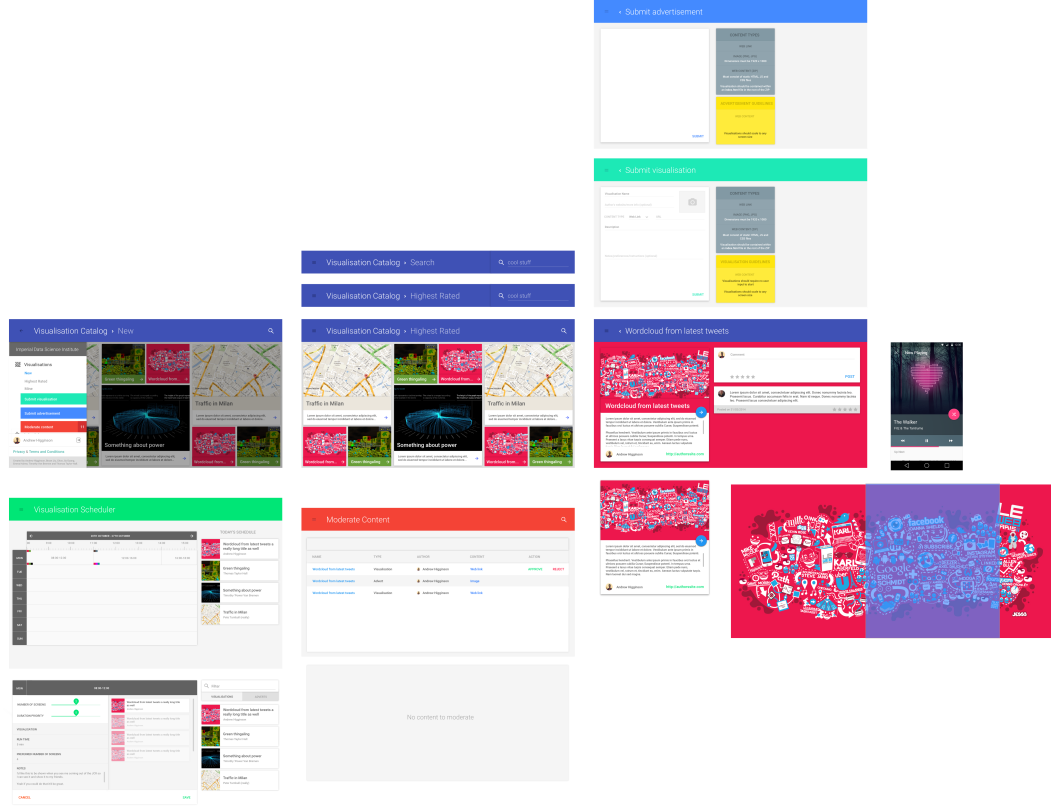
\includegraphics[width = \textwidth, trim = 0 0 0 0cm, clip]{./evaluation/mockup.png}
   \end{center}
   \caption{Mockups on User Interface}
   \label{fig:mockup}
\end{figure}

\subsection{Requirements on intangible ideas}
Compared to User Interfaces which user can see and feel, we believe 
uncovering the client's assumption on playout scheduling via mockups or 
prototypes would not be feasible as the algorithm is mainly rule-based.
We instead deliver our ideas with illustrations on whiteboard and
capture feedback from our supervisor.

Throughout discussions we have uncovered several assumptions, with one of them
expecting the scheduling algorithm to ensure playout time is 
directly proportional to metric set by administrators. In response,
we have created additional unit tests to incorporate such requirements 
in our scheduling algorithm.

\begin{figure}[H]
  \begin{minipage}{0.46\textwidth}
      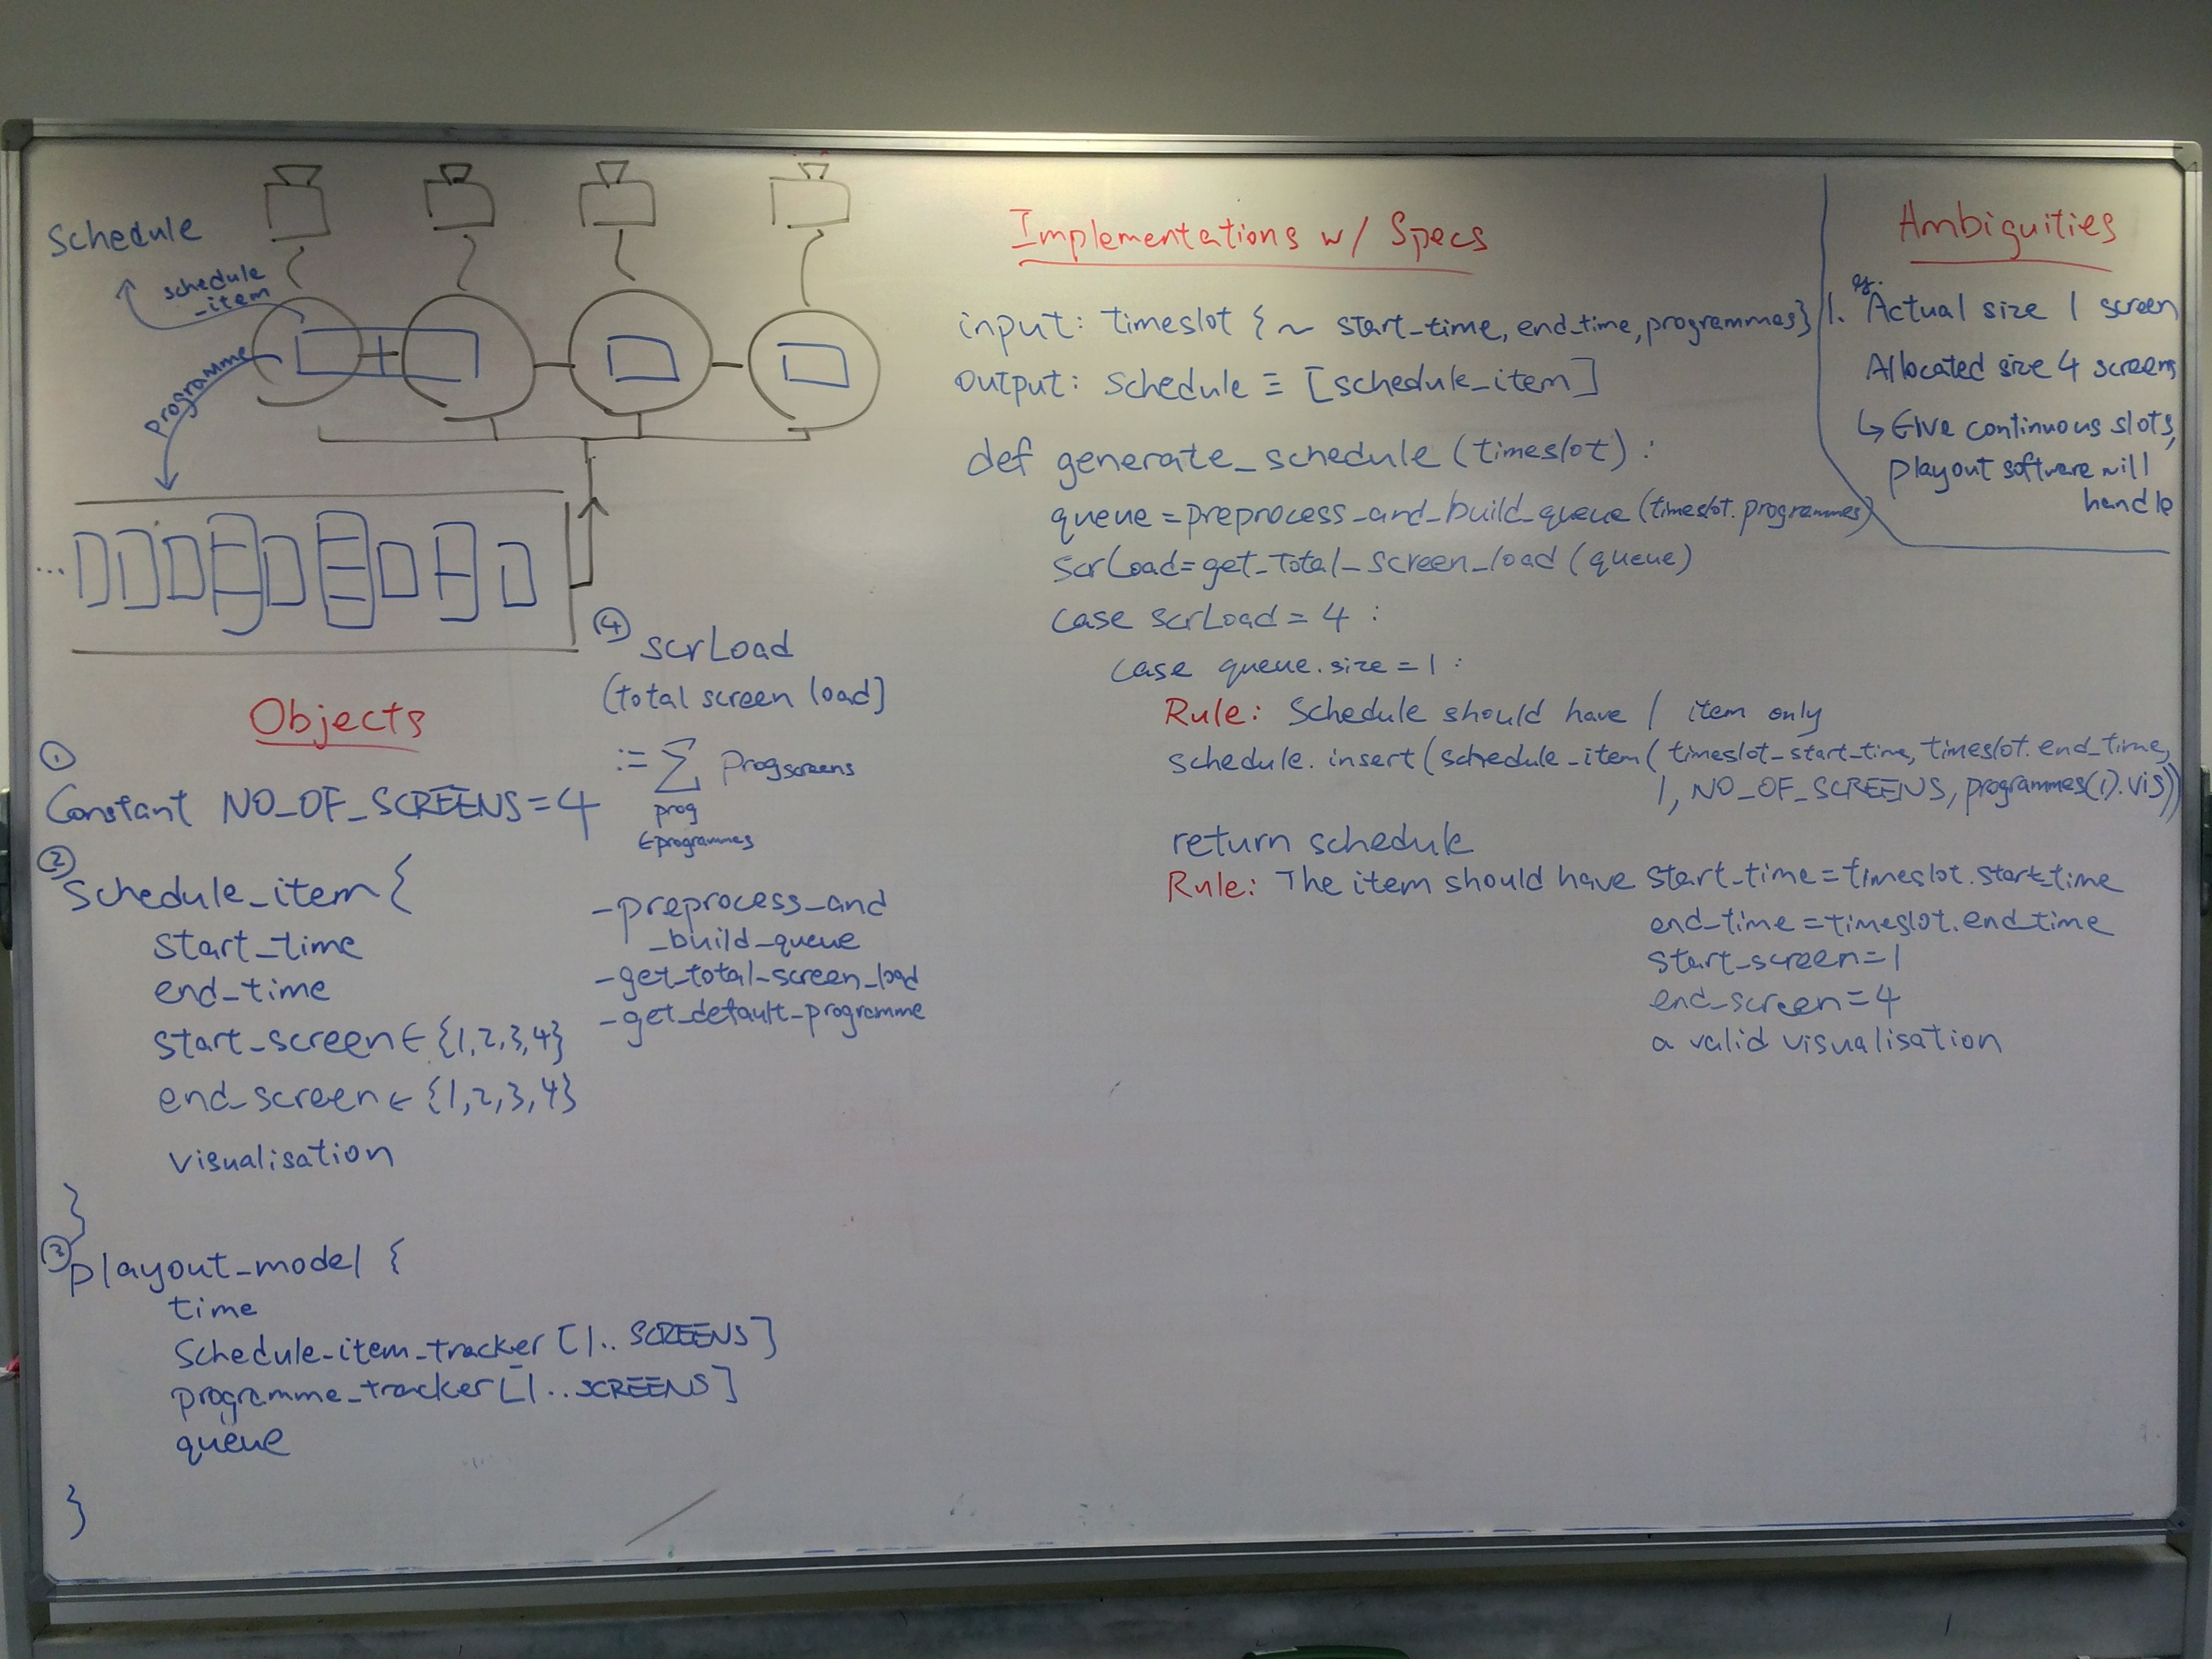
\includegraphics[width = 0.99\textwidth, trim = 0 1cm 0 1.5cm, clip]{./evaluation/scheduling_whiteboard.jpg}
  \end{minipage}
  \begin{minipage}{0.53\textwidth}
      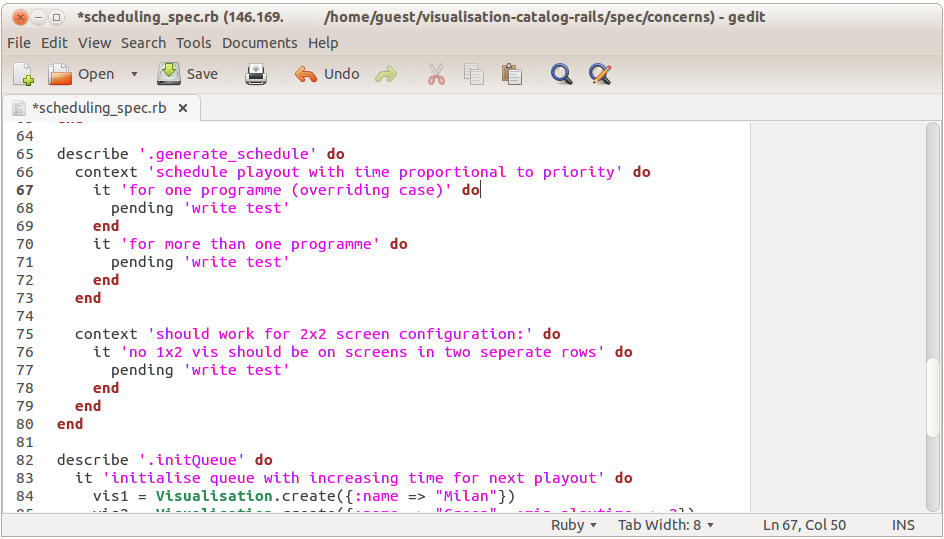
\includegraphics[width = 0.99\textwidth]{./evaluation/scheduling_spec.png}
  \end{minipage}
  \caption{Capturing scheduling requirements on whiteboard (left)\\ and subsequently via RSpec unit tests (right)}
 
\end{figure}

\subsection{User testing}
We have also conducted implicit user tests during demonstrations of new features,
where we ask our supervisor to conduct a task with minimal instruction and guidance
(e.g. to navigate to the visualisation scheduling page and schedule some visualistions
for playout).

Such testing allows us to learn what are obvious to us but obscure to users.
For example, in one of our demonstrations we observed that our supervior 
made multiple pauses when
being asked to navigate to the moderation and scheduling pages. This 
indicates the icon to show the user menu might not be evident to users and
description for menu items might not be clear enough. Based on such observations
we have changed the size of the ``show menu" button, as well as explored the effect
of different link colours on user menu.

We are planning to extend the user to test to cover more users, including staff
and students who would potentially use the platform to submit and view visualisations, the second in our list of stakeholders.

\section{Evaluation of Project}
%How will we evaluate?
As a group, we are constantly evaluating our project by testing after a 
feature is implemented. We make use of both RSpec and manual testing. In 
addition, our project progress is evaluated by David in our weekly 
meetings. Using Jenkins for Continuous Integration, we have given David
the address of our ``release vm'', where he can see the latest working 
version of the project. From this, David can constantly evaluate our project 
through all stages of development.

Quantitively, we can evaluate our project by ticking off our intial 
requirements. Also, we will use the systems ourselves, both from the user 
and administrator perspective, to evaluate the project from both our stakeholders.
This will include uploading of visualisations and viewing other visualisations as a
user, and moderating and scheduling visualisations as an admin.

Using our Trello board and version control, we can see which features have been 
implemented by which group member. To improve our teamwork for future group 
projects, we will sit down as a group and describe our strengths and weaknesses in 
this project.

TODO: get externals to evaluate, people from data science institute? 

TODO: stuff from eval lecture





\end{document}
